%\emph{System Level Description (Block diagram + description of 1 to 2 pages).}

%\emph{(Make sure that your description justifies how the Requirements of your system are met, especially those which are not obvious.)}

%% Remove the text above

This chapter will describe the system main blocks, the functionality of each of them, and the interaction between each block and its adjacent modules. Presented below (Figure \ref{fig:overview}) is a graphical overview of the system and its first layer of modules. A high resolution version is also included in \emph{Appendix \ref{app:overview}: System Overview}.

\begin{figure}[H]
  \centering
  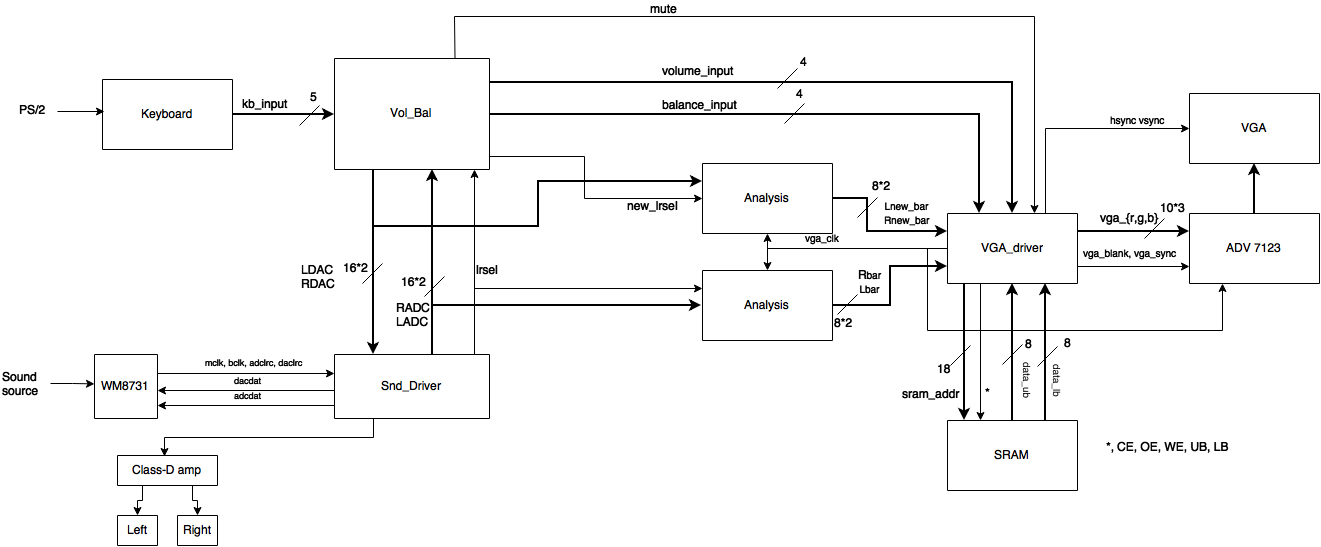
\includegraphics[scale=.18]{overview}
  \caption{A graphical overview of the system's first module layer. Letters inside curly braces indicates multiple signals exlusively including each of the letters.}
  \label{fig:overview}
\end{figure}

\section{Keyboard}\label{sec:keyboard}
The user interacts with the system through a PS/2-connected keyboard. The keyboard is then handled by the module \verb?Keyboard? which reads the scan codes, matches these against a \emph{one hot encoded} preset which makes up the \verb?kb_input? signal passed to \verb?Vol_Bal?.

The module inputs are \verb=PS2_DAT=, \verb=PS2_CLK=, \verb=clk= and \verb=rstn= which are used to shift in the scan code and compare the result with the preset, resulting in \verb=kb_input= --- a 2-bit unsigned value indicating if either of the arrow keys have been released. \verb=Vol_Bal= will then use this signal to adjust the volume and balance level. The Up/Down arrow keys controls the volume, and the Left/Right arrow keys controls the stereo channel balance.


\section{Snd\_Driver}\label{sec:snddriver}
The \verb?Snd_Driver? module is an audio signal coder/decoder. It translates the signal between a parallel format and a bit serial format. The parallel format is sent to the \verb?Vol_Bal? module which processes the sound and sends it to the class-D amplifier. The bit serial format is used by the WM8731 chip and the amplifier. This module will be a complete copy of the module used in \emph{Laboration 4}. In this case the module \verb?Vol_Bal? will replace and expand the \verb?Application? used in that laboration.

\begin{figure}[H]
  \centering
  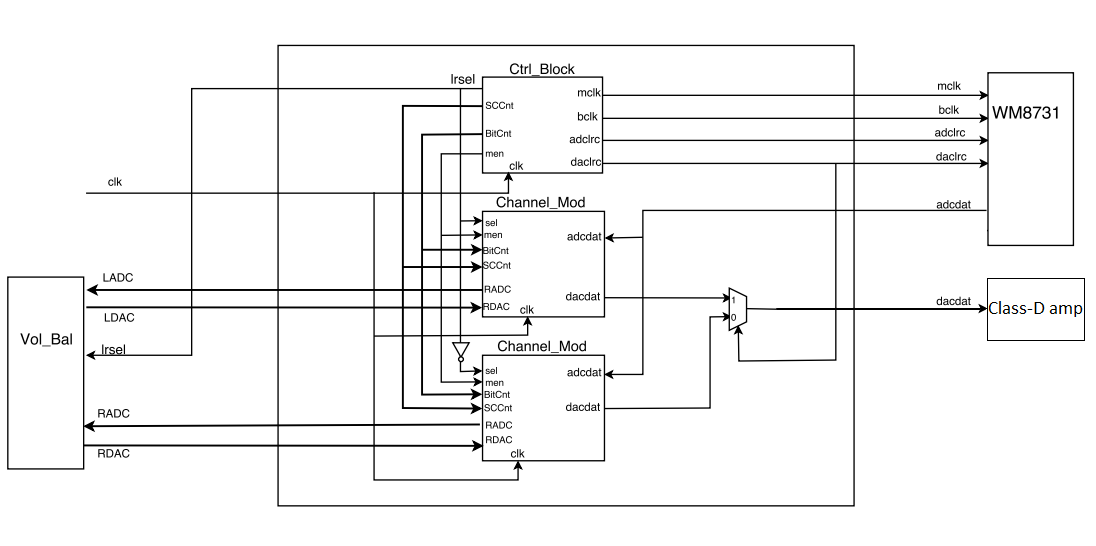
\includegraphics[scale=.40]{snddriver}
  \caption{The \texttt{Snd\_Driver} schematic, as seen in Lab 4, Audio Codec.}
  \label{fig:sndDriver}
\end{figure}


\section{Vol\_Bal}\label{sec:volbal}
The Volume/Balance module (\verb=Vol_Bal=) acts as the hub for processing incoming digital audio signals, forwarded from WM8731 via the \verb=Snd_Driver= module. As such, \verb=Vol_Bal= also keeps internal registers in the module \verb=Current_Vol_Bal= that holds volume (4-bit unsigned) and balance levels (4-bit signed), as well as a mute signal (std\_logic). These registers update via the one-hot coded input signal \verb=kb_input= applied by the \verb=Keyboard= module. Consequently, the values they hold are not only used as signals (\verb=i_volume_lvl=, \verb=i_balance_lvl=, \verb=i_mute=) for the internal submodule that process the \verb=LADC= and \verb=RADC= inputs, but also as module outputs connected to the \verb=VGA_Driver= so that they can be rendered on the screen.

\begin{figure}[h]
  \centering
  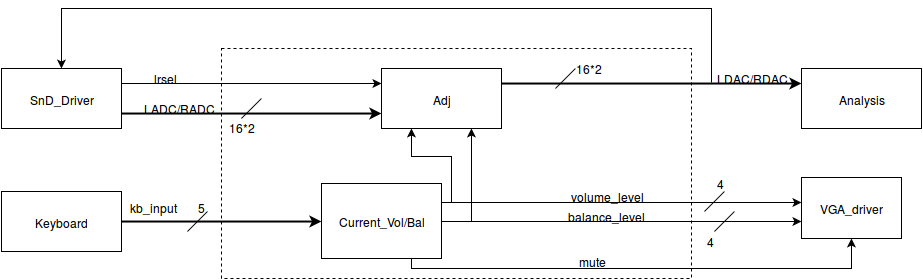
\includegraphics[width=16cm]{volbal}
  \caption{An overview of the Vol\_Bal module's internal workings.}
  \label{fig:vol_bal}
\end{figure}

The main function of the Volume/Balance module is to make requested adjustments to incoming values \verb=LADC= and \verb=RADC=, which represent measured amplitudes of the sound signal at distinct times. The sound will be adjusted for volume and balance by the functions:

\verb=   =$$A_{l\_new} = A_{l\_old} \cdot (1/\sqrt{2})^{n + m}\qquad\ ,\ m = 0\ for\ m < 0$$
\verb=   =$$A_{r\_new} = A_{r\_old} \cdot (1/\sqrt{2})^{n + |m|}\qquad,\ m = 0\ for\ m > 0\ ,$$

where $A$ is the amplitude, $n$ the volume level and $m$ the balance. \verb=lrsel= is used as a control signal for selecting the channel and the correct function. Resulting outputs \verb=LDAC= and \verb=RDAC= are forwarded to \verb=Snd_Driver= and to one instance of the \verb=Analysis= modules.

Ultimately, the user have the ability to digitally adjust the input sound by decreasing the volume in 3 dB decrements, down to -30 dB, and additionally regulate balance bias by further reducing volume by up to another 15 dB on a single left/right audio channel. There is also a mute function which is conveyed by \verb=kb_input=. When active, the register driving the \verb=mute= signal essentially blanks any $A_{new}$ values on the \verb=LDAC/RDAC= outputs.




\section{Analysis}\label{sec:analysis}
\begin{frame}
  \frametitle{Analysis}
	\begin{itemize}
		\item Analyzes incoming samples, low-pass filtering them.
		\item Output in form of a natural number, which determines the height of the bars.
		\item Updates in synd with vsync.
		\item Both left & right channel separately.
	\end{itemize}
\end{frame}

\begin{frame}
  \frametitle{Analysis}
	\begin{figure}[h]
		\centering
			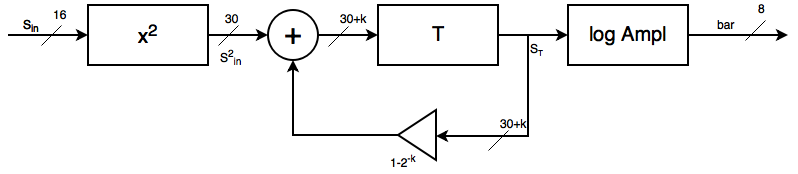
\includegraphics[width=16cm]{lowpass}
			\caption{The low-pass filter. $k$ is chosen by the approximation $\frac{1}{10}\mathrm{\ s} = 2^k\cdot\frac{1}{48800}\Rightarrow 2^k=4880\approx 2^{12}\Rightarrow k = 12 $}
			\label{fig:lowpass}
\end{figure}
\end{frame}


\section{VGA\_driver}\label{sec:vgadriver}
The \verb+vga_drive+ module exists to handle the rendering of a 640x480 resolution image on the screen. 
The image that is supposed to be rendered consists of a background image previously 
stored in the SRAM consisting of pre filled bars that within the module will be blanked
out according to the input stimuli, which will give the appearance of bars being filled 
to different levels.   

To render an image on the vga screen you need five main signals. Three analog color channels (red, green and blue)
and two signals for synchronization hsync and vsync. The image is rendered pixel by pixel line by line using
a horizontal sweep pattern which is reset by the two sync signals. If a color is set when the sweep resets
arbitrary patterns can occur and therefore the signal has to be blanked during the reset phase.

The module \verb+vga_drive+ has four input signals described in 

\begin{figure}[h]
        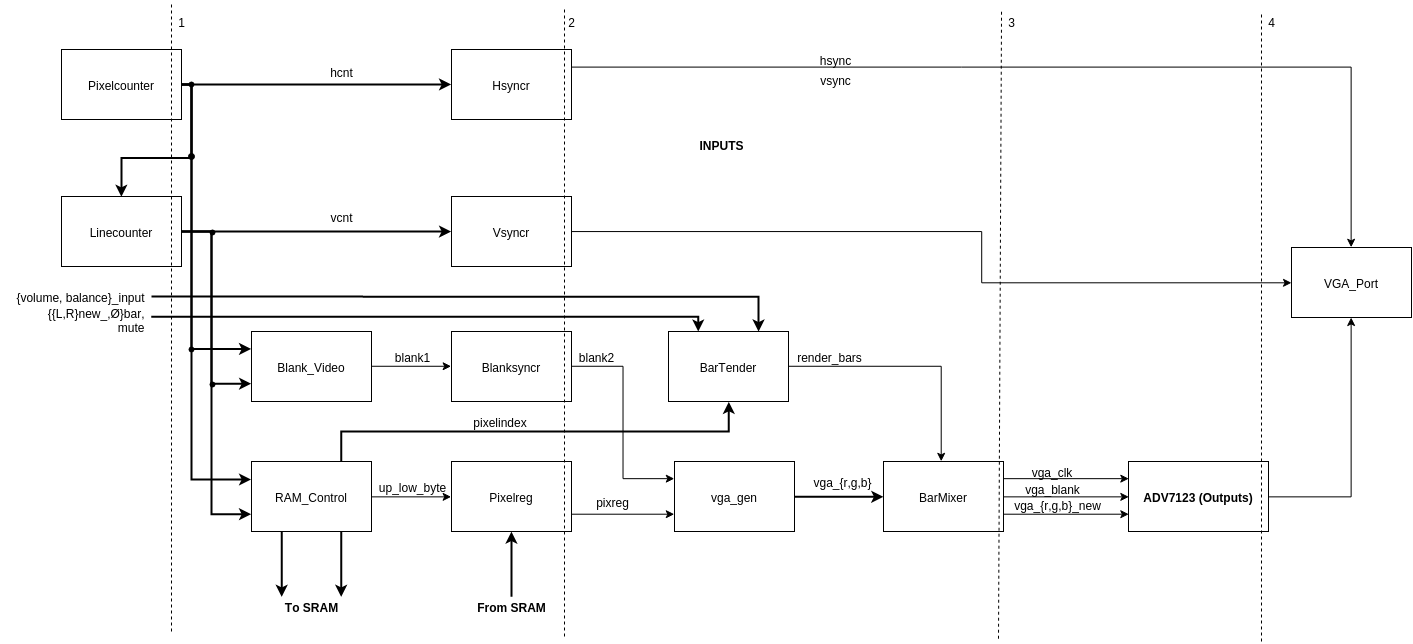
\includegraphics[scale=0.35]{vgadrive.png}
        \caption{Block diagram of vga\_drive}
        \label{fig:vgadrive}
\end{figure}

\begin{figure}[h]
        \caption{List of input signals}
        \label{tab:input}
\begin{tabular}{|r|l|}
        \hline
        \multicolumn{2}{|c|}{Input signals}\\
        \hline
        \multicolumn{1}{|c}{Name} & \multicolumn{1}{c|}{Description} \\
        \hline
        volume\_input & a 4 bit input containing volume information\\
        \cline{1-2}
        \hline
        balance\_input & a 4 bit input containing balance information\\
        \cline{1-2}    
        \hline
        bar & a n bit input containing signal sound input signal level\\
        \cline{1-2}    
        \hline
        new\_bar & a n bit input containing manipulated input signal level\\
        \cline{1-2}    
        \hline
\end{tabular}
\end{figure}

\begin{figure}[h]
        \caption{List of output signals}
        \label{tab:outputs}
\begin{tabular}{|r|l|}     
        \hline
        \multicolumn{2}{|c|}{output signals}\\
        \hline
        \multicolumn{1}{|c}{Name} & \multicolumn{1}{c|}{Description} \\
        \hline
        vga\_clk & clock signal needed for scanning\\
        \cline{1-2}
        \hline
        vga\_blank & a blanking signal for blanking when reseting scan\\
        \cline{1-2}    
        \hline
        vga\_(r,g,b) & three signals containing color information\\
        \cline{1-2}    
        \hline
\end{tabular}
\end{figure}

  \subsection{VGA\_driver:bartender}
  \subsection{VGA\_driver:barmixer}



